% Experiment E, 36 recorded observations (6 in each condition).
% A database-unavailable outcome is an operational failure, not a semantic rejection.
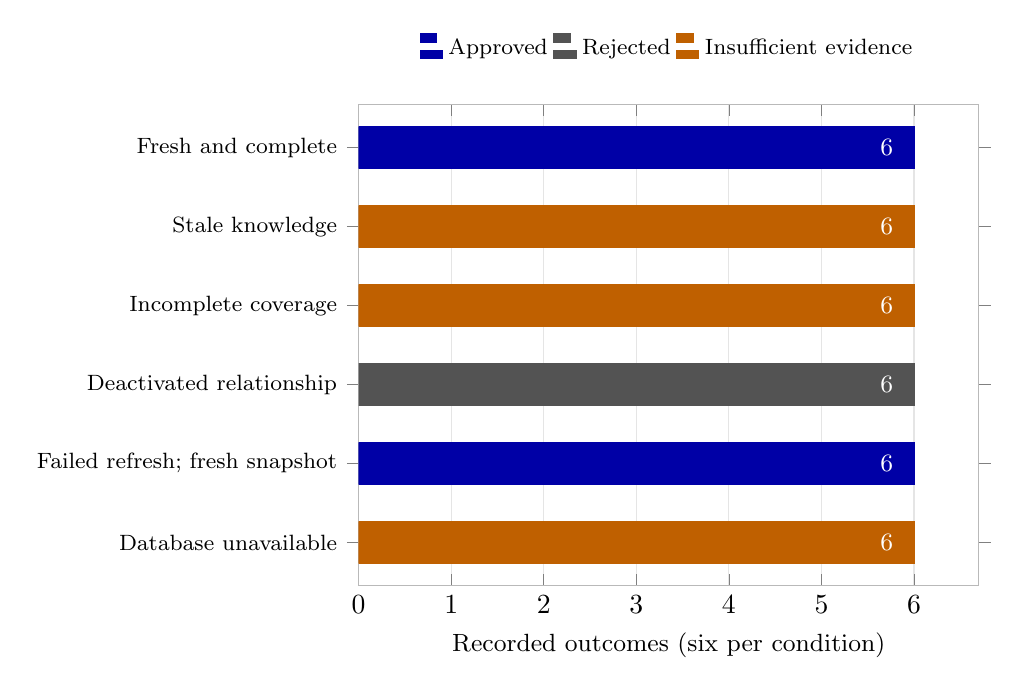
\begin{tikzpicture}
\begin{axis}[
    width=0.78\linewidth,
    height=7.7cm,
    xbar,
    xmin=0, xmax=6.7,
    ymin=0.45, ymax=6.55,
    xtick={0,1,2,3,4,5,6},
    ytick={1,2,3,4,5,6},
    yticklabels={Database unavailable,Failed refresh; fresh snapshot,Deactivated relationship,Incomplete coverage,Stale knowledge,Fresh and complete},
    yticklabel style={font=\footnotesize,align=right},
    xlabel={Recorded outcomes (six per condition)},
    xlabel style={font=\small},
    xmajorgrids=true,
    ymajorgrids=false,
    grid style={gray!20},
    axis line style={gray!55},
    legend style={font=\footnotesize,draw=none,at={(0.5,1.07)},anchor=south,legend columns=3},
    nodes near coords,
    every node near coord/.append style={font=\small,anchor=east,xshift=-4pt,text=white},
]
\addplot+[xbar,bar width=15pt,bar shift=0pt,
    fill=blue!65!black,draw=blue!65!black] coordinates {(6,6) (6,2)};
\addlegendentry{Approved}
\addplot+[xbar,bar width=15pt,bar shift=0pt,
    fill=gray!65!black,draw=gray!65!black] coordinates {(6,3)};
\addlegendentry{Rejected}
\addplot+[xbar,bar width=15pt,bar shift=0pt,
    fill=orange!75!black,draw=orange!75!black] coordinates {(6,5) (6,4) (6,1)};
\addlegendentry{Insufficient evidence}
\end{axis}
\end{tikzpicture}
